\chapter{Elección de la Tecnología}

\section{¿Por que Web y no Desktop?}

Una aplicacion Desktop (tambien llamada de Escritorio) es aquella que requiere
ser instalada en el Ordenador (PC) del Usuario, y que es ejecutada directamente
por el sistema operativo, ya sea Microsoft Windows, GNU/Linux, Mac OS, etc.

Algunos Ejemplos de Estas Aplicaciones:

\begin{itemize}
    \item Winamp
    \item Adobe Photoshop
    \item iTunes
    \item Microsoft Oficce (Word, Excel, Power Point. etc)
\end{itemize}

Aunque suelen ser mas robustas y estables que las aplicaciones Web Presentan
varios inconvenientes tales como:

\begin{itemize}
    \item Su acceso solo se limita al ordenandor donde fue instalada.
    \item La Aplicacion es dependiente del Sistema Operativo que utilice el ordenador, aunque
        existen programas Multiplataforma no aseguran una compatibilidad completa.
    \item Requieren una instalacion personalizada
    \item En caso de Actualizaciones requieren que estas se hagan de forma manual en cada ordenador
        donde se instalo la Aplicacion.
    \item Suelen Tener requerimientos especiales de Software y librerias para poder funcionar.
\end{itemize}


Una aplicacion Web, es aquella que solo requiere ser instalada en un Servidor, su 
ejecucion requiere unicamente Disponer de un ordenador con conexíon a internet
y un navegador en contraparte de las Desktop que requiere que se instale en cada 
ordenador donde se pretende usar.

Por lo cual brinda una serie de ventajas tales como:

\begin{itemize}
    \item Portabilidad, se ejecuta desde cualquier ordenador que posea coneccion a internet sin
        depender de Software adicional, Plataforma y/o Sistema Operativo.
    \item La informacion que se maneja es multiusuario por lo que son especialmente utiles para
        desarrollar aplicaciones multiusuarios basadas en compartir informacion.
    \item Consumen muy pocos recursos, por lo que el usuario no necesita tener un ordenador con 
        grandes prestaciones para trabajar con ellas.
    \item Son faciles de Actualizar y mantener.
    \item Se pueden utilizar en miles de equipos sin limitacion y restriccion alguna.
    \item Su funcionalidad es independiente del Sistema Operativo Instalado en el ordenador del 
            usuario.
    \item No hay problemas de incompatibilidad de Version de software ya que los usuarios trabajan 
        con la misma version.
\end{itemize}
En resumen el Sistema por sus caracteristicas podria haberse implementado como un sistema
Deskop pero se ubiesen perdido las caracteristicas deseadas del mismo.

%%%%%%%%%%%%%%%%%%%%%%%%%%%%%%%%%%%%%%%%%%%%%%%%%%%%%%%%%%%%%%%%%%%%%%%%%%%%%%%%

\section{Apache}

El servidor HTTP Apache es un servidor web HTTP de código abierto, para plataformas
Unix (BSD, GNU/Linux, etc.), Microsoft Windows, Macintosh y otras, que implementa
el protocolo HTTP/1.12 y la noción de sitio virtual. Cuando comenzó su desarrollo en 1995 se basó inicialmente
en código del popular NCSA HTTPd 1.3, pero más tarde fue reescrito por completo. Su nombre se
debe a que Behelendorf quería que tuviese la connotación de algo que es firme
y enérgico pero no agresivo, y la tribu Apache fue la última en rendirse al que pronto se
convertiría en gobierno de EEUU, y en esos momentos la preocupación de su grupo era que
llegasen las empresas y "civilizasen" el paisaje que habían creado los primeros ingenieros de internet.
Además Apache consistía solamente en un conjunto de parches a aplicar al servidor de NCSA.
En inglés, a patchy server (un servidor "parcheado") suena igual que Apache Server. 

El servidor Apache se desarrolla dentro del proyecto HTTP Server (httpd) de la
Apache Software Foundation.

Apache presenta entre otras características altamente configurables, bases de
datos de autenticación y negociado de contenido, pero fue criticado por la falta
de una interfaz gráfica que ayude en su configuración.\\[0.2cm]

\section{mod\_wsgi}

mod\_wsgi es un módulo de Apache que provee una interfaz WSGI para correr
 Web en Python sobre Apache. Y esto, es todo lo que necesitas para que tus
 archivos *.py se ejecuten por medio de un navegador Web.

\subsection{WSGI}

WSGI es el acronomico de Web Server Gateway Interface que es una especificacion
para una simple y universal interfaz entre una aplicacion web (en nuestro caso
una aplicacion escrita en Django) y un servidor Web para el lenguaje de programacion
Python. Es un estandar de Python el cual se describe con detalle en la PEP 333
\footnote{\url{http://www.python.org/dev/peps/pep-0333/}}


%%%%%%%%%%%%%%%%%%%%%%%%%%%%%%%%%%%%%%%%%%%%%%%%%%%%%%%%%%%%%%%%%%%%%%%%%%%%%%%%

\section{PosgreSQL}

PostgreSQL es un gestor de base de datos relacional que puede correr tanto bajo
sistemas operativos Windows como en distribuciones Linux como Red Hat, Suse,
Centos, etc.

Como muchos otros proyectos de código abierto, el desarrollo de PostgreSQL
no es manejado por una empresa y/o persona, sino que es dirigido por una comunidad
de desarrolladores que trabajan de forma desinteresada, altruista, libre y/o
apoyados por organizaciones comerciales. Dicha comunidad es denominada
el PGDG (PostgreSQL Global Development Group).

El nombre hace referencia a los orígenes del proyecto como la base de datos
"post-Ingres", y los autores originales también desarrollaron la base de datos Ingres.

El proyecto post-ingres pretendía resolver los problemas con el modelo de base
de datos relacional que habían sido aclarados a comienzos de los años 1980. El
principal de estos problemas era la incapacidad del modelo relacional de
comprender "tipos", es decir, combinaciones de datos simples que conforman una
única unidad. Actualmente estos son llamados objetos. Se esforzaron en introducir
la menor cantidad posible de funcionalidades para completar el soporte de tipos.
Estas funcionalidades incluían la habilidad de definir tipos, pero también
la habilidad de describir relaciones - las cuales hasta ese momento eran
ampliamente utilizadas pero mantenidas completamente por el usuario. En Postgres
la base de datos «comprendía» las relaciones y podía obtener información de
tablas relacionadas utilizando reglas. Postgres usó muchas ideas de Ingres
pero no su código.

%%%%%%%%%%%%%%%%%%%%%%%%%%%%%%%%%%%%%%%%%%%%%%%%%%%%%%%%%%%%%%%%%%%%%%%%%%%%%%%%

\section{Python}

Django esta escrito puramente en Python, por lo que Obiamente Necesitaremos Instalar
Python. Python es un lenguaje de programación interpretado cuya filosofía hace
 hincapié en una sintaxis muy limpia y que favorezca un código legible.
 
Se trata de un lenguaje de programación multiparadigma, ya que soporta
orientación a objetos, programación imperativa y, en menor medida, programación
funcional. Es un lenguaje interpretado, usa tipado dinámico y es multiplataforma.

Es administrado por la Python Software Foundation. Posee una licencia de código
abierto, denominada Python Software Foundation License,1 que es compatible con
la Licencia pública general de GNU a partir de la versión 2.1.1, e
incompatible en ciertas versiones anteriores.

Python es un lenguaje de programación multiparadigma. Esto significa que más
que forzar a los programadores a adoptar un estilo particular de programación,
permite varios estilos: programación orientada a objetos, programación imperativa
y programación funcional. Otros paradigmas están soportados mediante el uso
de extensiones.

Python usa tipado dinámico y conteo de referencias para la administración
de memoria.

Una característica importante de Python es la resolución dinámica de nombres;
 es decir, lo que enlaza un método y un nombre de variable durante la ejecución
  del programa (también llamado enlace dinámico de métodos).
  
Otro objetivo del diseño del lenguaje es la facilidad de extensión. Se pueden
escribir nuevos módulos fácilmente en C o C++. Python puede incluirse en
aplicaciones que necesitan una interfaz programable.

Aunque la programación en Python podría considerarse en algunas situaciones
hostil a la programación funcional tradicional del Lisp, existen bastantes
analogías entre Python y los lenguajes minimalistas de la familia Lisp como
puede ser Scheme.

\subsection{La Filosofia detras de Python}
Los usuarios de Python se refieren a menudo a la Filosofía Python que es bastante
análoga a la filosofía de Unix. El código que sigue los principios de Python de
legibilidad y transparencia se dice que es "pythonico". Contrariamente, el
código opaco u ofuscado es bautizado como "no pythonico" ("unpythonic" en inglés).

Estos principios fueron famosamente descritos por el desarrollador de Python Tim
Peters en El Zen de Python, algunos de ellos son:

\begin{itemize}
    \item Bello es mejor que feo.
    \item Explícito es mejor que implícito.
    \item Simple es mejor que complejo.
    \item Complejo es mejor que complicado.
    \item Plano es mejor que anidado.
    \item Disperso es mejor que denso.
    \item La legibilidad cuenta.
    \item Los casos especiales no son tan especiales como para quebrantar las reglas.
    \item Aunque lo práctico gana a la pureza.
    \item Los errores nunca deberían dejarse pasar silenciosamente.
    \item A menos que hayan sido silenciados explícitamente.
    \item Frente a la ambigüedad, rechaza la tentación de adivinar.
    \item Debería haber una y preferiblemente sólo una manera obvia de hacerlo.
    \item Aunque esa manera puede no ser obvia al principio a menos que usted sea holandés.15
    \item Ahora es mejor que nunca.
    \item Aunque nunca es a menudo mejor que ya mismo.
    \item Si la implementación es difícil de explicar, es una mala idea.
    \item Si la implementación es fácil de explicar, puede que sea una buena idea.
    \item Los espacios de nombres (namespaces) son una gran idea ¡Hagamos más de esas cosas!
\end{itemize}


\subsection{Baterias Incluidas}

Python tiene una gran biblioteca estándar, usada para una diversidad de tareas.
Esto viene de la filosofía "pilas incluidas" ("batteries included") en referencia
a los módulos de Python. Los módulos de la biblioteca estándar pueden mejorarse por
módulos personalizados escritos tanto en C como en Python. Debido a la gran
variedad de herramientas incluidas en la biblioteca estándar, combinada con la
habilidad de usar lenguajes de bajo nivel como C y C++, los cuales son capaces
de interactuar con otras bibliotecas, {\bfseries Python es un lenguaje que combina su clara
sintaxis con el inmenso poder de lenguajes menos elegantes}.

\subsection{Implementaciones}

En la actualidad existen diversas implementaciones de Python

\begin{itemize}
    \item {\bfseries CPython} es la implementación original, disponible para varias plataformas en el sitio oficial de Python.
    \item {\bfseries IronPython} es la implementación para .NET
    \item {\bfseries Stackless Python} es la variante de CPython que trata de no usar el stack de C \url{www.stackless.com}
    \item {\bfseries Jython} es la implementación hecha en Java
    \item {\bfseries Pippy} es la implementación realizada para Palm \url{pippy.sourceforge.net}
    \item {\bfseries PyPy} es una implementación de Python escrita en Python y optimizada mediante JIT \url{pypy.org}
\end{itemize}

%%%%%%%%%%%%%%%%%%%%%%%%%%%%%%%%%%%%%%%%%%%%%%%%%%%%%%%%%%%%%%%%%%%%%%%%%%%%%%%%

\section{Django}


Django es un framework de desarrollo web de código abierto, escrito en Python,
que respeta el paradigma conocido como {\bfseries Model Template View}. Fue desarrollado en
origen para gestionar varias páginas orientadas a noticias de la
{\bfseries World Company de Lawrence, Kansas}, y fue liberada al público bajo una licencia
BSD en julio de 2005; el framework fue nombrado en alusión al guitarrista de
jazz gitano Django Reinhardt \url{http://es.wikipedia.org/wiki/Django_Reinhardt}.

En junio del 2008 fue anunciado que la recién formada Django Software Foundation
se haría cargo de Django en el futuro.

La meta fundamental de Django es facilitar la creación de sitios web complejos.
Django pone énfasis en el re-uso, la conectividad y extensibilidad de
componentes, el desarrollo rápido y el principio No te repitas
(DRY, del inglés Don't Repeat Yourself). Python es usado en todas las partes
del framework, incluso en configuraciones, archivos, y en los modelos de datos.


\subsection{MVC}

Antes de Explicar como funciona Django empezare por una breve explicacion de
el patr\'on (MVC) Modelo Vista Controlador el cual es un patrón de arquitectura de software que
separa los datos y la lógica de negocio de una aplicación de la interfaz de
usuario y el módulo encargado de gestionar los eventos y las comunicaciones.
Para ello MVC propone la construcción de tres componentes distintos que son el
modelo, la vista y el controlador, es decir, por un lado define componentes
para la representación de la información, y por otro lado para la interacción
 del usuario. Este patrón de diseño se basa en las ideas de reutilización de
 código y la separación de conceptos, características que buscan facilitar la
 tarea de desarrollo de aplicaciones y su posterior mantenimiento.

De manera genérica, los componentes de MVC se podrían definir como sigue:

{\bfseries  El Modelo:} Es la representación de la información con la cual el sistema opera,
por lo tanto gestiona todos los accesos a dicha información, tanto consultas
como actualizaciones, implementando también los privilegios de acceso que se
hayan descrito en las especificaciones de la aplicación (lógica de negocio).
Envía a la 'vista' aquella parte de la información que en cada momento se le
solicita para que sea mostrada (típicamente a un usuario). Las peticiones de
acceso o manipulación de información llegan al 'modelo' a través del
'controlador'.

{\bfseries El Controlador: } Responde a eventos (usualmente acciones del
usuario) e invoca peticiones al 'modelo' cuando se hace alguna solicitud sobre
la información (por ejemplo, editar un documento o un registro en una base de
datos). También puede enviar comandos a su 'vista' asociada si se solicita un
cambio en la forma en que se presenta de 'modelo' (por ejemplo, desplazamiento
 o scroll por un documento o por los diferentes registros de una base de datos),
  por tanto se podría decir que el 'controlador' hace de intermediario entre
   la 'vista' y el 'modelo' actuando como Middleware
\footnote{Middleware es el software que proporciona un enlace entre aplicaciones de software
independientes. Middleware a veces se llama a la vía que conecta dos
aplicaciones y pasa los datos entre ellas. Los Middleware permiten que los
datos contenidos en una base de datos puedan ser accedidos a través de otra.
Ahorra el tiempo a los programadores.}.
   
{\bfseries La Vista: } Presenta el 'modelo' (información y lógica de negocio)
 en un formato adecuado para interactuar (usualmente la interfaz de usuario)
 por tanto requiere de dicho 'modelo' la información que debe representar como
 salida.

\begin{figure}[h]
    \centering
    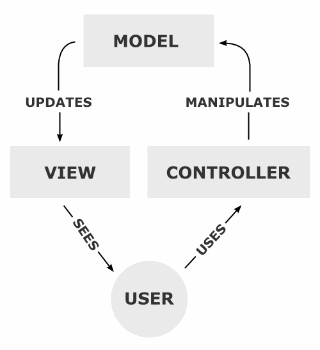
\includegraphics[scale=0.7]{resourse/MVC-Process.png}
    \caption{Diagrama del Patron MVC Modelo Vista Controlador}
    \label{fig:03}
\end{figure}    


\subsection{Django y el MVT}

Si hicieramos una clasificacion de Herramientas de desarrollo web, podriamos
clasificar a Django como parte de la tercera generacion:


\begin{figure}[h]
    \centering
    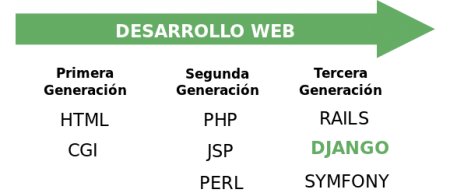
\includegraphics[scale=0.7]{resourse/desarrolloweb.png}
    \caption{Generaciones de Herramientas de Desarrollo Web}
    \label{fig:02}
\end{figure}   

Sin embargo más alla de las clasificaciones que podr\'ian existir, está el
entender como funciona realmente, al entenderlo se puede llegar a dominarlo.

Dijimos que era un framework MTV (una modificación de MVC, nada que ver con
un canal de m\'usica), esto se debe a que los desarrolladores no tuvieron la
 intención de seguir algún patron de desarrollo, sino hacer el framework lo
más funcional posible.

\begin{itemize}
    \item {\bfseries  El Modelo} en Django sigue siendo el modelo
    \item {\bfseries La Vista} en Django se llama Plantilla (Template)
    \item {\bfseries El controlador} en Django se llama Vista
\end{itemize}

Una imagen nos hará entender mejor esta relación:

\begin{figure}[h]
    \centering
    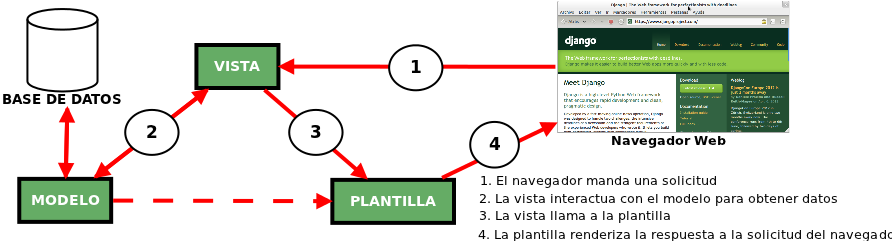
\includegraphics[scale=0.5]{resourse/esquema-mtv.png}
    \caption{El patron Modelo Vista Template de Django}
    \label{fig:04}
\end{figure}   



\subsection{El Modelo}

El modelo define los datos almacenados, se encuentra en forma de clases de
Python, las clases definidas son traducidas por Django y este genera las Tablas
necesarias para el funcionamiento del modelo dentro de la base de datos, cada
tipo de dato que debe ser almacenado se encuentra en una variable 
con ciertos parámetros, posee métodos también. Todo esto permite indicar y
controlar el comportamiento de los datos.\\[0.1cm]

Aqui un extracto del codigo mostrando como se implementa uno de los tantos
modelos con los que trabaja el Sistema\\[0.3cm]


\begin{lstlisting}[style=Python]

class Message(models.Model):
    """
        Clase Para Manejar mensajes entre usuarios
    """
    from_user = models.ForeignKey(User, related_name='from_user')
    to_user = models.ForeignKey(User, related_name='to_user')
    date = models.DateTimeField("Fecha y Hora",auto_now_add=True)
    issue = models.CharField("Asunto",max_length=125, default='')
    content = models.TextField("Cuerpo del Mensaje")
    read = models.BooleanField("Leido",default=False)


    class Meta:
        db_table = "Messages"
        verbose_name = "InboxMessage"
        verbose_name_plural = "InboxMessages"
\end{lstlisting}

\footnote{Como algunos lo notaran la variable from\_user del modelo internamente
es una relacion 1:M dentro de la base de datos.}

\footnote{La Clase interna Meta define atributos expeciales como 'db\_name' que hace
referencia a como se llamara la tabla dentro de la Bases de Datos.}

\vspace{0.1cm}

\subsection{La Vista}
La vista se presenta en forma de funciones en Python, su propósito es
determinar que datos serán visualizados, entre otras cosas más que iremos
viendo conforme avanzamos con el curso. El ORM de Django permite escribir
código Python en lugar de SQL para hacer las consultas que necesita la vista.
La vista también se encarga de tareas conocidas como el envío de correo
electrónico, la autenticación con servicios externos y la validación de
datos a través de formularios. Lo mas importante a entender con respecto a la
 vista es que no tiene nada que ver con el estilo de presentación de los
 datos, sólo se encarga de los datos, la presentación es tarea de la plantilla.\\[0.1cm]


Aqui muestro una vista sencilla que realiza una consulta base de datos que listara todos
los usuarios que sean medicos. \\[0.1cm]

\begin{lstlisting}[style=Python]
def patient_show_medics_list(request):
    """
        Muestra el listado de Medicos
    """
    mi_template = get_template('Patients/GestionTurnos/medics-list.html')
    dict = generate_base_keys(request)

    if is_patient(request.user):
        dict['medics'] = UserInformation.objects.filter( \\
                                    user__groups__name='Medico')
        html_cont = mi_template.render(Context(dict))
        return HttpResponse(html_cont)

    else:
        #si hay un usuario logueado intentanto acceder sera enviado a una
        # pagina de error
        path = request.META['PATH_INFO']
        return HttpResponseRedirect("/restricted-access%s" %path)
\end{lstlisting}

\vspace{0.1cm}

Aunque es un ejemplo sencillo podemos apreciar el potencial de Django, como vemos
no vemos ningun codigo SQL, pues bien dicho codigo SQL se ejecuta internamente
nos aleja del problema de las restriciones de la Base de Datos ya sea que usemos
PosgreSQL (como en este sistema), MySQL, SQLServer o SQLite nosotros
solo escribiremos codigo Python, El framework se encargargara de traducir esa
instrucion al motor de bases de datos correspondiente que estemos usando.\\[0.2cm]

\begin{lstlisting}[style=consola]
dict['medics'] = UserInformation.objects.filter( \\
                            user__groups__name='Medico')
\end{lstlisting}

\vspace{0.1cm}

Traducido a SQL terminariamos con algo tan orrible como esto:\\[0.1cm]

\begin{lstlisting}[style=consola]
SELECT * FROM UserInformation as Info
INNER JOIN User ON Info.username = User.username
INNER JOIN GroupsByUsers ON User.username = GroupsByUsers.username
...
\end{lstlisting}

\vspace{0.1cm}

\subsection{La Plantilla}
La plantilla es básicamente una página HTML con algunas etiquetas extras
propias de Django, en si no solamente crea contenido en HTML (también XML, CSS,
Javascript, CSV, etc).\\[0.1cm]

La plantilla recibe los datos de la vista y luego los organiza para la
presentación al navegador web. Las etiquetas que Django usa para las plantillas
permiten que sea flexible para los
diseñadores del frontend, pueden Extenderse a partir de otras plantillas incluso
tiene estructuras de datos como if, por por si es necesaria una presentación
lógica de los datos, estas estructuras
son límitadas para evitar un desorden poniendo cualquier tipo de código Python.\\[0.1cm]

Esto permite que la lógica del sistema siga permaneciendo en la vista. Aqui la
vista para Iniciar Session:\\[0.1cm]

\begin{lstlisting}[style=HTML]



<link type="text/css" rel="stylesheet" media="all"
    href="/media/css/fancy-forms.css" />
<link type="text/css" rel="stylesheet" media="all"
    href="/media/css/gradient-buttons.css" />
<link type="text/css" rel="stylesheet" media="all"
    href="/media/css/messages.css" />




<br /><br /><br />
        
            <div class="fancy-form-white" style="width: 350px;
                margin: 0 auto;">
                <h3 class="title">Inciar Session</h3><br />
                <form action="." method="POST">
                <table style="margin: 0 auto; width: 330px;" >
                <tr>
                    <td><label for="username">Usuario:</label></td>
                    <td><input type="text" name="username" value=""
                    tabindex="1" id="username"></td>
                    <td rowspan="2">
                    <input type="submit" value="Login" tabindex="3"
                    class="grad-button-blue" style="height: 50px;">
                    </td>
                </tr>
                <tr>
                    <td><label for="password">Contrase\~na:</label></td>
                    <td><input type="password" name="password" value=""
                     tabindex="2" id="password"></td>
                </tr>
                </table>
                </form>
                <br />
            </div>

            
                    <br />
                    <br />
                <div class="alert">Alerta: Error Usuario y/o Contrase\~na
                Incorrectos</div>
            

        
            <div class="alert">Alerta: Usted ya ha iniciado session con el
            usuario <strong>{{ username }}</strong></div>
            <br />
            <a href="/logout">Cerrar Session</a>
        

\end{lstlisting}

\vspace{0.1cm}

\subsection{La Configuracion de Rutas}

Django posee un mapeo de URLs que permite controlar el despliegue de las vistas,
esta configuración es conocida como URLConf. El trabajo del URLConf es leer
la URL que el usuario solicitó, encontrar la vista apropiada para la solicitud
y pasar cualquier variable que la vista necesite para completar su trabajo. El
URLConf esta construido con expresiones regulares en Python y sigue la filosofia
de Python: Explicito es mejor que implícito. Este URLConf permite que las rutas
que maneje Django seán agradables y entendibles para el usuario.\\[0.1cm]

Fragmento del archivo urls.py del Proyecto\\[0.1cm]

\begin{lstlisting}[style=HTML]
    (r'^$', base_views.index),
    (r'^index/$', base_views.index),
    (r'^login/$', base_views.login),
    (r'^logout/$', base_views.logout),
    (r'^change-password/$', base_views.change_password),
    (r'^restricted-access/$', base_views.restricted_access),
    (r'^restricted-access/(.+)/$', base_views.restricted_access),
\end{lstlisting}

\vspace{0.1cm}
